\subsection{Example call}
\label{sec:example-call}
In this section we provide the sequence of calls between the architectural components when the first requirement of \ref{par:asrs} is implemented: \textit{The system should be able to retract relevant information  from the xml files that are created by the users of OptaPlanner}.\\\\
Starting with the highest-level component, the API uses the \verb!SolverFactory! to create different solver instances. 
In this class there is one method called \verb!createFromXmlResource! which is responsible for setting up the solver based on the \verb!xml! configuration files. It implements this by using a class called \verb!solverConfig! which is an instantiation of the \verb!SolverConfig! class from the Configuration system. 
The \verb!SolverConfig! class makes use of the \verb!DefaultSolver! class from the Implementation system. The relationship is established in the \verb!buildSolver! method which returns a new instance of the \verb!DefaultSolver! class. A graphical representation of this can be noted in figure \ref{fig:example-call}. 
\subsection{Difference with Step 1}
In this section we will briefly explain the difference between the architectural model that we established in this step of the assignment as opposed to the one we established in step 1 (\S\ref{subsec:arch-comp}). In the top-down model we assumed that an important architectural component of the system would be one that is concerned with handling the configuration specifications of the \verb!xml! files. This assumption was correct because we were able to discern that one of the main architectural components of OptaPlanner is the Configuration system.\\\\
The other three components that we assumed about in step 1 are also crucial entities of the system, however they are not defined as main architectural components. Instead, they are concepts that are implemented in the Configuration and Implementation systems, or as we have sometimes referred to, sub-components of the main architectural components.
% EXAMPLE CALL
\begin{figure}
    \centering
    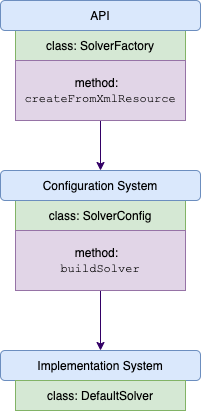
\includegraphics[width=0.3\textwidth]{figures/example-call.png}
    \caption{In this figure we depict a graphical representation of the dependency relationships between the three architectural components in \S \ref{sec:example-call}. The arrow flow is downward which means that the start of the arrow is the dependent class.}
    \label{fig:example-call}
\end{figure}